\documentclass[a4paper,12pt]{article}
\usepackage[utf8]{inputenc}%%seul package à charger : pour éviter les problèmes sordides d'encodage
\usepackage[fiche, psc]{andre}%%bon eh bien sûr...
\usepackage{wrapfig}
%%fiche, psc pour faire une fiche
%%rapport, psc pour faire un rapport
%%pour insérer du code : \langage{java} , puis \begin{lstlisting} \end{lstlisting}
%%pour insérer des guillemets : \eg \og

\title{Projet Scientifique Collectif X2013 \\INF02~: Synthétiseur automatique de documents}

\renewcommand{\petittitre}{Projet INF02}
\author{Fernandes-Pinto-Fachada Sarah, Schrottenloher Andr\'e, Angibault Antonin,\\
Hufschmitt Th\'eophane, Cao Zhixing, Boisseau Guillaume}

\date{24 avril 2015}

\begin{document}

%\titrelong%%une page complète
\titrecourt %titre plus court, typiquement pour les fiches

\subsection*{Contacts}

\begin{itemize}
 \item \textbf{Antonin Angibault} (chef de projet)~: \href{mailto:antonin.angibault@polytechnique.edu}{antonin.angibault@polytechnique.edu} ;
 \item \textbf{Théophane Hufschmitt}~: \href{mailto:theophane.hufschmitt@polytechnique.edu}{mailto:theophane.hufschmitt@polytechnique.edu}.
\end{itemize}


\subsection*{Résumé}

Notre projet a pour ambition \textbf{d'analyser sémantiquement un texte}, de manière automatique, afin de produire un \textbf{résumé} de celui-ci. \\

\begin{wrapfigure}{r}{10cm}
  \centering
  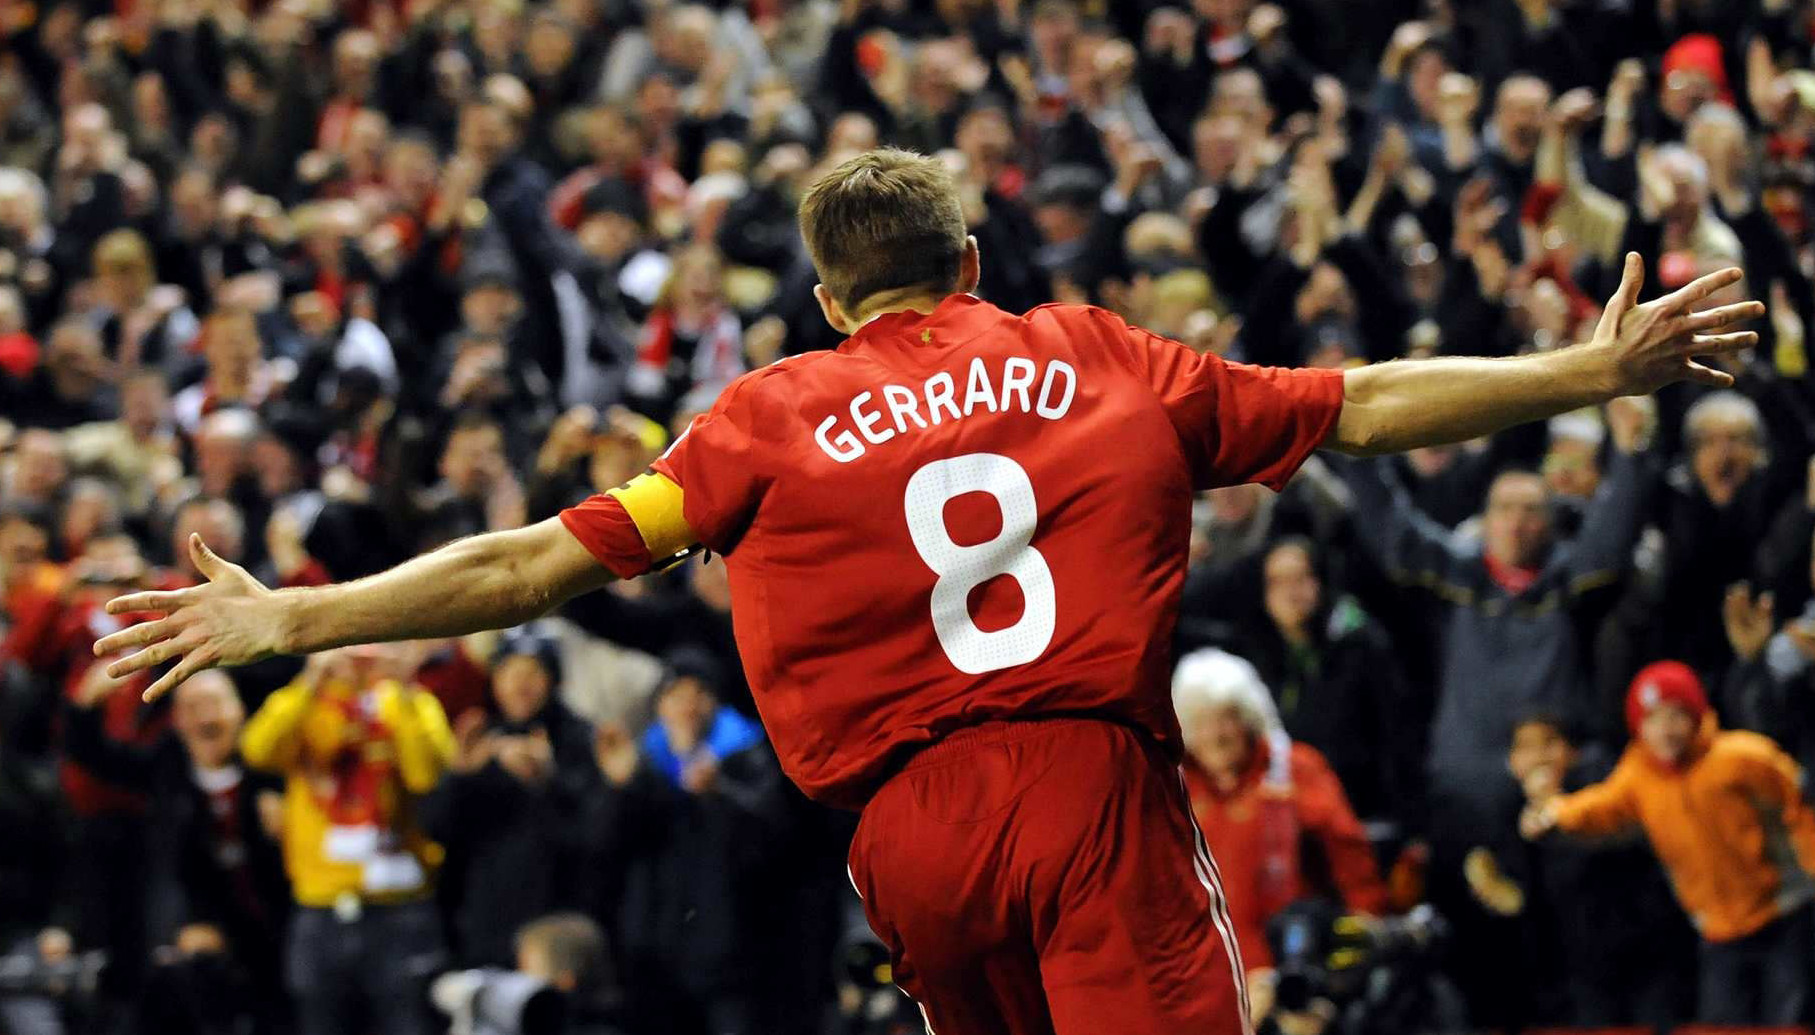
\includegraphics[width = 10cm]{./gerrard.jpg}
\end{wrapfigure}

Les méthodes actuelles de résumé automatique se tournent en grande partie vers les outils statistiques : fréquences d'apparition de mots, sélection de mots-clés. Sans pour autant nous départir de la manipulation de grandes quantités de données textuelles, nous essayons d'introduire un véritable facteur de \textbf{compréhension du texte}, en manipulant des informations sémantiques ; qui sont porteuses d'un véritable sens. 

\begin{figure}[h]
 \centering
 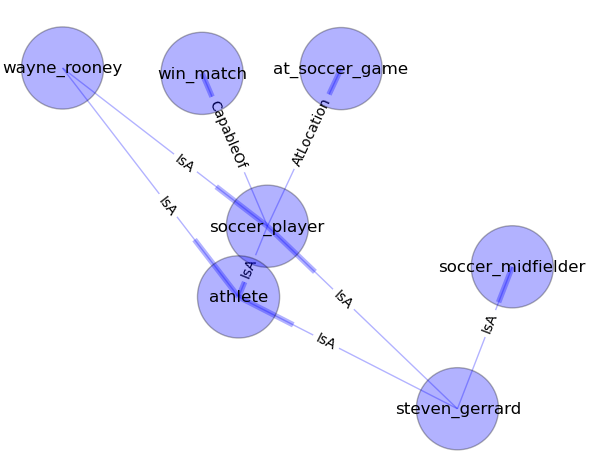
\includegraphics[width=10 cm]{./figure_1.png}
 % figure_1.png: 812x612 pixel, 100dpi, 20.62x15.54 cm, bb=0 0 585 441
% \caption{Représentation des données}
\end{figure}


%Ce point de vue original nous a amenés à explorer différents sous-problèmes, de l'analyse syntaxique à la représentation de données sémantiques en passant par l'introduction de structures de données malléables, dans le but d'y reconstruire l'information du texte et d'y sélectionner les informations pertinentes recherchées.



 
\end{document}



